\documentclass{neu_handout}
\usepackage{url}
\usepackage{amssymb}
\usepackage{amsmath}
\usepackage{marvosym}
\usepackage{graphicx}
\usepackage[pdftex]{graphicx}
\usepackage{subfigure}
\graphicspath{ {images/} }
\everymath{\displaystyle}

% Professor/Course information
\title{Milestone 1 - UFOs}
\author{Abby, Emily, Lydia and Peter (The Conspiracists)}
\date{March 2018}
\course{CS 7295}{Information Visualization}

\begin{document}

\section*{1 Data acquisition and clean-up}

\textbf{How dirty was the data and what kind of clean-up was required? How
easy was it to download / use API? What is the format of the data? What are the
items and attributes in your dataset? What types of data are you working with
(categorical, ordinal, quantitative)?}\\

We acquired the data easily from the Reporting Database of the National UFO Reporting Center's website\footnote{Raw Data: \url{https://drive.google.com/open?id=1x9nxzOGCApOaGvbX1Mv2wh83-ZRfidR-}}. The reports are organized in tables which can be accessed by the following indices: Event Date, State, Shape, Date Posted. When organized by dates, the website provides one table for each month. We downloaded the tables for each month of 2017 into one excel sheet. Since the report form of the website mostly provides the user with a specific set of options for each question, the data set was relatively clean. The attributes of each item, i.e. report, are:

\begin{description}
  \item[$\bullet$ Date] (date and time of sighting) - quantitative
  \item[$\bullet$ City] (city and/or area of the sighting) - categorical
  \item[$\bullet$ State] - categorical
  \item[$\bullet$ Shape] (one of the 21* choices for craft shapes) - categorical
  \item[$\bullet$ Duration] (statement of estimated duration of the sighting in text) - quantitative
  \item[$\bullet$ Summary] (written description and comments on the sighting)
  \item[$\bullet$ Date Posted] (date the report was posted) - quantitative
\end{description}

We note that there are missing values in the attributes Shape and Duration. We only kept the reports regarding sightings in the US since there were only a few reports outside the US and we can assume that these areas would not be well represented. After this, we are left with 4593 reports. We fixed a few obvious mistakes on the states probably caused by miss-clicking the state close to the right one on the drop-down menu. We changed all the craft shapes with value "Unknown" to missing values, assuming that a missing value and an "Unknown" value essentially mean the same thing. Finally, since we intend to use Duration as a quantitative attribute, we used the information of the text to derive the duration of the sighting in minutes. For this last part, we used the mean of a range to give a single number of minutes and we had to make some assumptions as to what people perceive as "a few minutes" or "several hours" for example. We believe that these assumptions do not alter the data significantly and would not affect our visualizations.


\section*{2 Exploring the data}

\textbf{Any interesting
trends/observations? Any evidence of missing or “dirty” data? Any features or
observations in the data that are confusing or unexpected?}\\

We explored our data in Tableau and Google Explore. We noticed that there are particular dates with a higher number of UFO sightings, such as Dec 22, Jul 4, Dec 9, and Jan 1. Some of these reports could have been caused by celebratory events associated with certain holidays. For the vast majority of the reports, the sighting's duration was at most one hour but in general the range of the durations is very large (one second to 20 years). In addition, most sightings refer to objects with "Light" or "Circle" shape and all 20 shapes (except for "Unknown", which we cleaned) are present. This will probably make it difficult for us to represent this categorical variable. Finally, although the time of a sighting is almost a uniformly distributed variable, there were a lot of sightings occurring at exactly 3:00 am.\\

*Changing, Chevron, Cigar, Circle, Cone, Cross, Cylinder, Diamond, Disk, Egg, Fireball, Flask, Formation, Light, Other, Oval, Rectangle, Sphere, Teardrop, Triangle, Unknown


\section*{3 Interview}

\textbf{How did the interview go? What did you learn? What were you surprised by during the interview? Has the interview changed your motivating questions?}\\ 

After some initial trouble communicating with the director of the National UFO database, and trouble with sourcing a line of communication, we had a solid half hour interview with Peter Davenpor \footnote{Interview Notes: \url{https://docs.google.com/document/d/1ejWb30b9zhYVn6H0adOAkQ_ZRSgHtJb8noliHprtfIw/edit}}, Director of the National UFO Reporting Center. Davenport discussed with us many things regarding his database, most notable of which was his role in establishing the data collection method that the Center uses now. Davenport modernized the collection and organization of the data, both retroactively and for use in the future. I was surprised by how much the tone and attitude of the interview subject changed over the course of the scheduling process and interview; initially, Davenport was skeptical of our use of his data and interview. During the interview, it came to light that this was due to him being burned before by major publications and national news outlets. Our interview was incredibly informative but I do not believe that it changed our line of questioning or reasoning in this project.\\


\section*{4 Task analysis}

\textbf{Create a full list of “domain” tasks (i.e., what are the tasks a
user wants to accomplish with the data using your visualization) and translate these into high/mid/low level tasks.}

\begin{table}[h]
\caption{Domain Tasks} % title name of the table
\centering % centering table
\begin{tabular}{c c c} % creating 3 columns
\hline\hline % inserting double-line
 Task & Abstraction & Level \\ [0.5ex]
\hline % inserts single-line
Observe all UFO sightings of 2017 & 
Analyze/Consume/Discover & High \\[1ex] %space

Observe how the UFO \\sightings occur throughout the year &
Analyze/Consume/Present &
High \\[1ex] %space

Curiosity stimulation &
Analyze/Consume/Enjoy &
High \\[1ex] %space

Look for areas with high number of sightings &
Search/Explore &
Mid \\[1ex] %space


Are there clusters of UFO\\ sightings according to geographic area? &
Cluster &
Low  \\[1ex] %space

Learn details of sighting (e.g. time, shape, description) &
Retrieve Value &
Low \\[1ex] %space

Only see sightings of particular shape &
Filter &
Low \\[1ex] %space

When did the sightings of a particular area \\(e.g. my hometown) occur? &
Filter &
Low \\[1ex] %space

What state has the most sightings? &
Find Extremum &
Low \\[1ex] %space

What date has the most sightings? &
Find Extremum &
Low \\[1ex] %space

Capture the sightings of a particular month &
Analyze/Produce/Record &
High \\[1ex] %space

What is the distribution of the times\\ of the day the sightings occur? &
Characterize Distribution &
Low \\


\hline 
\end{tabular}
\label{tab:PPer}
\end{table}

\subsection*{4.2 Sketches}

\subsubsection*{Abby's}

\subsubsection*{Emily's}
\begin{figure}[h]
\centering
{
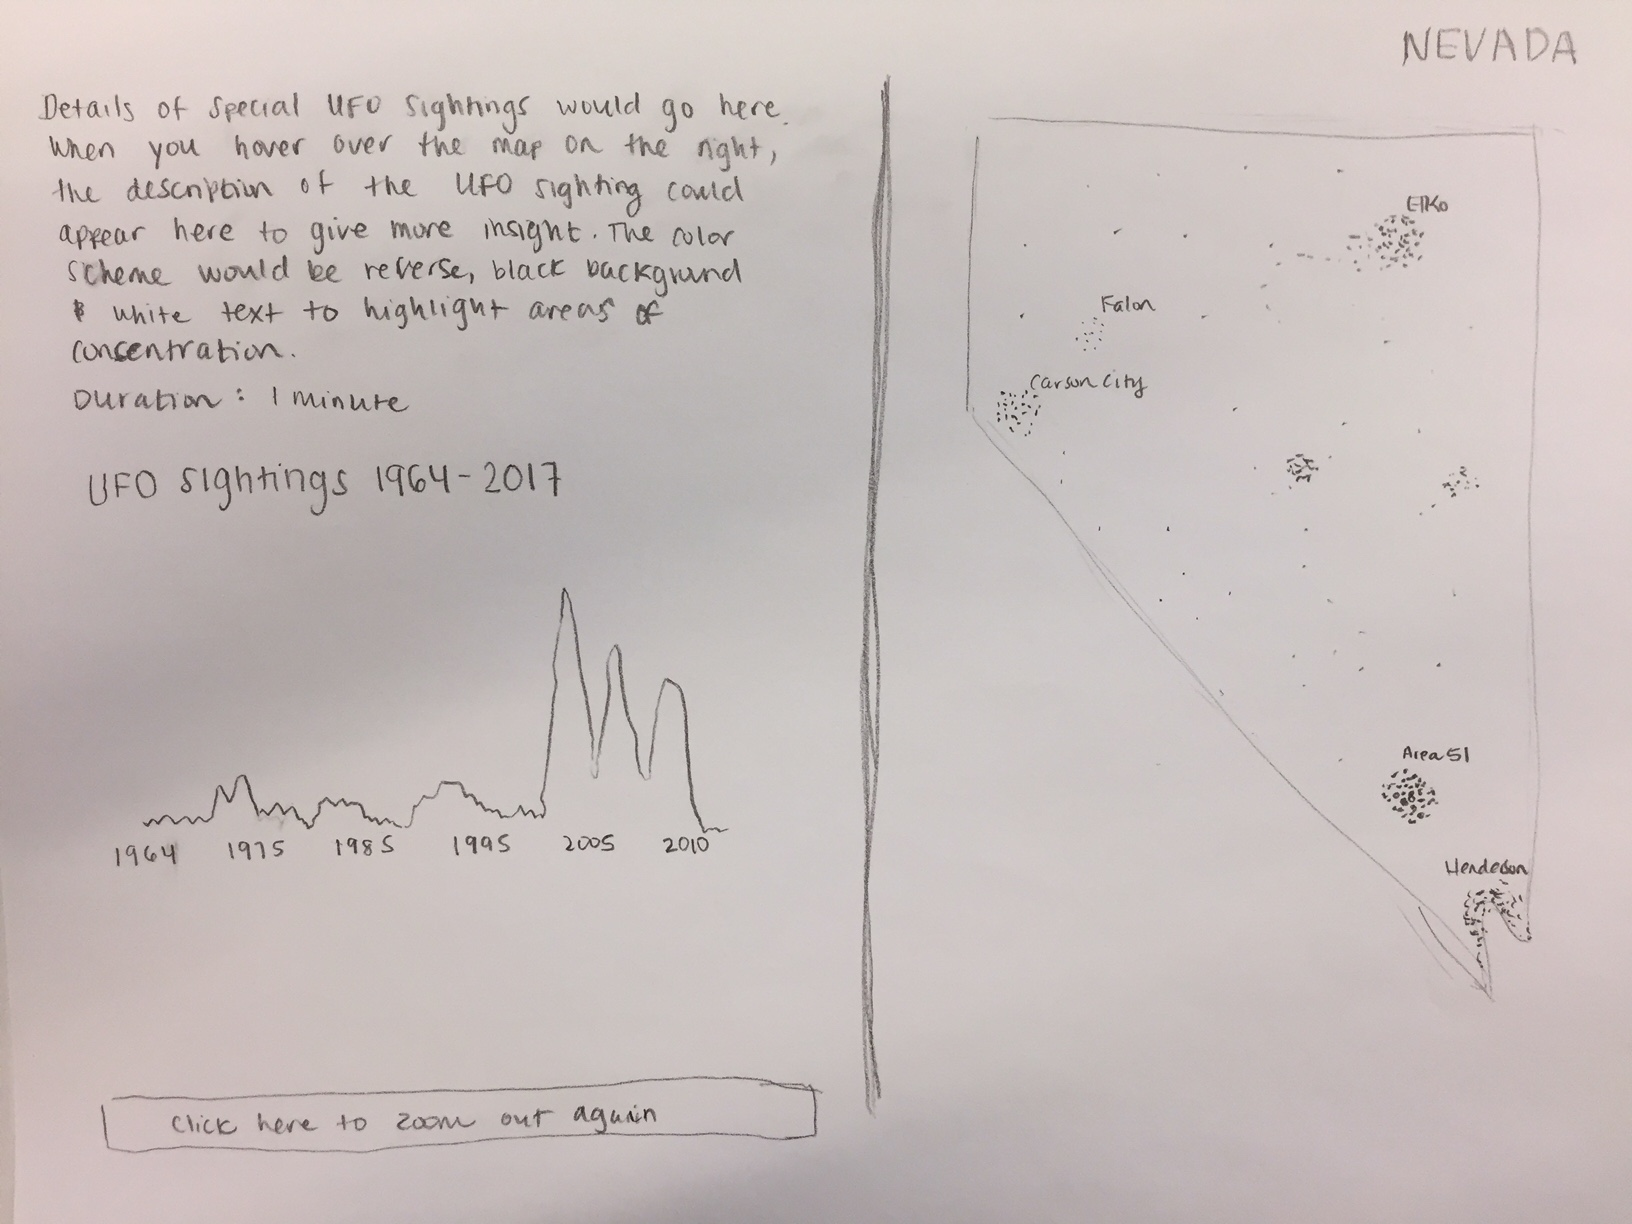
\includegraphics[width=0.5\linewidth]{emily1}
}
\end{figure}

The idea of this visualization would be able to allow users to select particular states in order to observe all UFO sightings by state. Filters could be provided in order to change the time series from all of the data points, to simply just 2017. A map will be used to highlight the number of UFO sightings (showing density), using a black background and white text and encoding to make the number of sightings pop. A line chart would be used to show the quantitative number of sightings, and the detailed description of the UFO sighting would be given above the line chart when a user hovers over a particular data point on the map.\\\\

\begin{figure}[h]
\centering
{
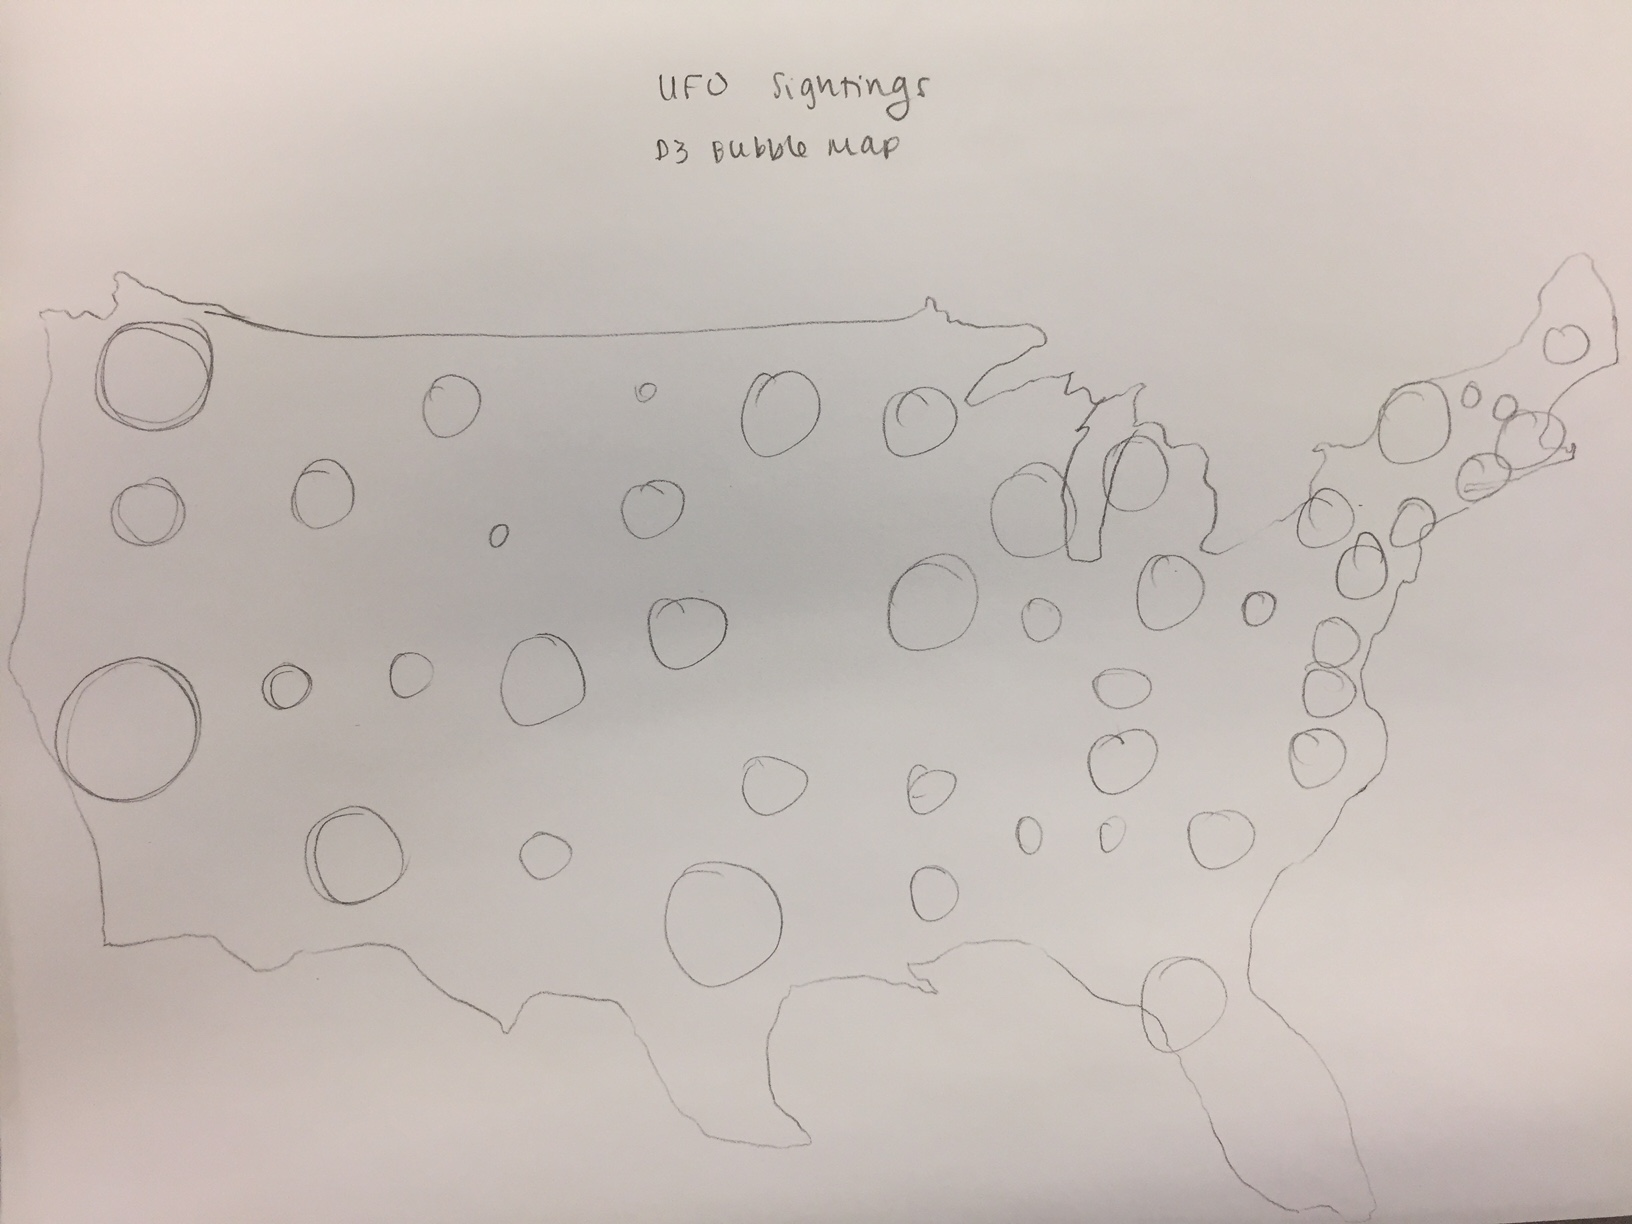
\includegraphics[width=0.5\linewidth]{emily2}
}
\end{figure}

This D3 bubble map would should the total number of reported UFO sightings in the United States by state over the last x number of years (the time range would ideally be filtered by the user). The bubbles would be in a light shaded color in order to make them stand out, and the size of the bubbles would be based upon the number of UFO sightings reported (i.e. 100, 1k, 5, 10k). A legend would be displayed as well.

\subsubsection*{Lydia's}

\subsubsection*{Peters's}


\end{document}
